\documentclass[12pt]{article}

\usepackage[a4paper,
            total={170mm,255mm},
            left=10mm,
            top=15mm]
            {geometry}

\usepackage{fontspec,
            polyglossia,
            graphicx}

\usepackage{amsmath,
            amsthm,
            amssymb}

\usepackage{unicode-math,
            tensor}

\usepackage{wrapfig,
            hyperref,
            multicol,
            multirow,
            tabularx,
            booktabs,
            subfiles}

\setdefaultlanguage{russian}
\setotherlanguage{english}
\setkeys{russian}{babelshorthands=true}

\defaultfontfeatures{Ligatures=TeX}
\setmainfont{STIX Two Text}
\setmathfont{STIX Two Math}
\DeclareSymbolFont{letters}{\encodingdefault}{\rmdefault}{m}{it}

\newfontfamily{\cyrillicfont}{STIX Two Text} 
\newfontfamily{\cyrillicfontrm}{STIX Two Text}
\newfontfamily{\cyrillicfonttt}{Courier New}
\newfontfamily{\cyrillicfontsf}{STIX Two Text}

\renewcommand{\thefigure}{\thesection.\arabic{figure}}
\renewcommand{\thetable}{\thesection.\arabic{table}}
\numberwithin{equation}{section}

\renewcommand{\qedsymbol}{$\blacksquare$}
\theoremstyle{definition}
\newtheorem{definition}{Опр.}[section]
\theoremstyle{remark}
\newtheorem{statement}{Утв.}[section]
\theoremstyle{plain}
\newtheorem{theorem}{Теор.}[section]

\graphicspath{{./img/}}
\everymath{\displaystyle}

\newcommand{\llabel}[1]{\label{\thesubsection:#1}}
\newcommand{\lref}[1]{\ref{\thesubsection:#1}}


\begin{document}
	\paragraph{48.}
	Рассмотрите задачу о потенциальном барьере конечной ширины.\\
	% Коммент для Артёма: я не ёб, как сделать норм каппу, поэтому вставил какую есть
	
	\textbf{Вся нижеследующая чушь будет для случая с порогом, потому что он является прелюдией к барьеру.}
	
	В любой потенциальной яме конечной глубины есть хотя бы один уровень. Чем глубже, тем больше уровней. Частицы, проходящие над ямой (не слишком высоко) - могут отражаться.
	
	\begin{equation*}
	V(x) = 
	\begin{cases}
	0 , x < 0 \\
	V_i , x > 0
	\end{cases}
	\end{equation*}
	\begin{wrapfigure}{L}{.4\linewidth}
	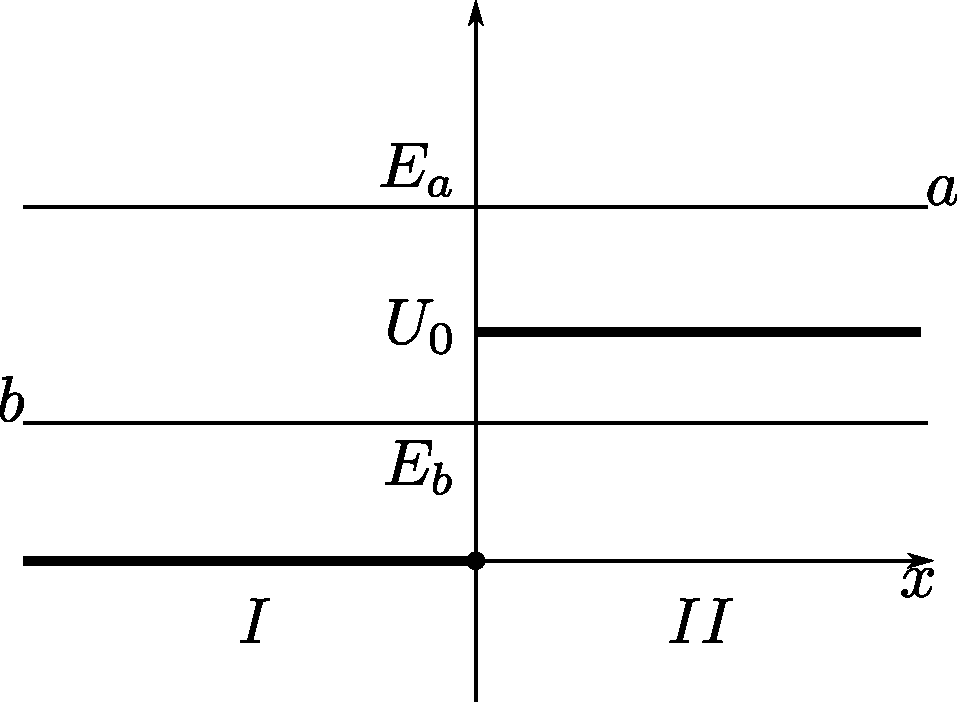
\includegraphics[width=1\linewidth]{48-01}
	\end{wrapfigure}
	Классическая механика: если $\xi < V_0$, то движение возможно лишь при $x < 0$; если $\xi > V_0$, то всюду, но $T_{\RNumb{2}} < T_{\RNumb{1}}$
	\\\\
	\textbf{Рассмотрим случай под кодовым названием А, где} $\xi > V_0$.
	
	Область $\RNumb{1} \ (x<0)$ : 
	
	$$\frac{\hbar}{2m} \frac{d^2 \psi}{dx^2} + \xi \psi = 0 \rightarrow \frac{d^2 \psi}{dx^2}+{k_1}^2 \psi = 0,$$
	
	где $k_1 = \frac{\sqrt{2m\xi}}{\hbar}$.
	
	$$\psi_{\RNumb{1}} = A_1 e^{i k_1 x} + B_1 e^{-i k_1 x}.$$
	
	Область $\RNumb{2} \ (x>0)$ :
	
	$$\frac{\hbar}{2m} \frac{d^2 \psi}{dx^2} + (\xi - V_0) \psi = 0 \rightarrow \frac{d^2 \psi}{dx^2}+{k_2}^2 \psi = 0,$$
	
	где $k_2 = \frac{\sqrt{2m(\xi - V_0)}}{\hbar}$.
	
	$$\psi_{\RNumb{2}} = A_2 e^{i k_2 x} + B_2 e^{-i k_2 x}.$$
	
	Допустим, что волна первоначалально набегает слева направо, а источника электронов на $+ \infty$ нет, тогда $B_\alpha = 0$.
	
	Из непрерывности $\psi(x)$ и $\frac{d\psi(x)}{dx}$ на границе $x = 0$:
	
	\begin{equation*}
	\begin{cases}
		\psi_{\RNumb{1}} (0) = \psi_{\RNumb{2}} (0) \\
		\psi'_{\RNumb{1}} (0) = \psi'_{\RNumb{2}} (0)
	\end{cases}
	\end{equation*}
	
	\begin{equation*}
	\begin{cases}
	 A_1 + B_1 = A_2 \\
	 ik_1 (A_1 - B_1) = i k_2 A_2
	\end{cases}
	\end{equation*}
	
	Откуда:
	
	$$(A_1 +B_1)k_2 = (A_1 - B_1)k_1 \rightarrow B_1 = \frac{k_1 - k_2}{k_1 + k_2} A_1 \ and \ A_2 = \frac{2 k_1}{k_1 +k_2} A_1$$
		
	Величина вектора плотности тока вероятности в области $\RNumb{1}$ есть:
	
	$$d_1 = \frac{\hbar k_1}{m} (| A_1 |^2 - | B_1 |^2)$$
	
	Величина вектора плотности тока вероятности в области $\RNumb{2}$ есть:
	
	$$d_2 = \frac{\hbar k_2}{m} | A_2 |^2$$
	
	Для стационарных состояний $\Delta \vec{j} = 0 \Rightarrow j_1 = j_2$
	
	$$k_1(|A_1|^2 - |B_1|^2) = k_2 |A_2|^2$$
	
	Коэффициент отражения характеризует вероятность отражения от порога: $R \equiv \frac{| B_1 |^2}{| A_1 |^2}$
	
	Коэффициент прохождения: $D \equiv \frac{k_2 | A_2 |^2 }{k_1 | A_1 |^2}$
	
	Суммарно они дают единицу.
	\\\\
	\textbf{Перейдём к случаю под кодовым названием Б, где} $\xi < V_0$.
	
	Область $\RNumb{1} \ (x<0)$ :
	 
	Всё так же как и в случае А: $\psi_{\RNumb{1}} = A_1 e^{i k_1 x} + B_1 e^{-i k_1 x}$
	
	Область $\RNumb{2} \ (x>0)$ :
	
	$$\frac{\hbar^2}{2m} \frac{x^2 \psi}{dx^2} + (\xi -V_0) \psi = 0 \rightarrow \frac{d^2 \psi}{dx^2} - \kappa^2 \psi = 0$$
	
	$$\kappa = \frac{\sqrt{2m(V_0 - \xi)}}{\hbar}$$ 
	
	$$\psi_{\RNumb{2}} = A_2 e^{\kappa x} + B_2 e^{-\kappa x}$$
	
	К дифуру, конечно, полагаются граничные условия:
	
	\begin{equation*}
		\begin{cases}
			\psi_{\RNumb{1}} (0) = \psi_{\RNumb{2}} (0) \\
			\psi'_{\RNumb{1}} (0) = \psi'_{\RNumb{2}} (0)	
		\end{cases}
	\end{equation*}

	\begin{equation*}
		\begin{cases}
			A_1 + B_1 = B_2 \\
			i k_1 (A_1 - B_1) = -\kappa B_2	
		\end{cases}
	\end{equation*}

	$$-\kappa (A_1 + B_1) = i k_1 (A_1 - B_1) \rightarrow B_1 = -\frac{\kappa + i k_1}{\kappa - i k_1} A_1 \ и \ B_2 = \frac{-2ik_1}{\kappa - i k_1} A_1 \rightarrow R = \frac{\kappa ^2+ k_1^2}{\kappa^2+k_1^2} = 1$$
	
	$$\psi_{\RNumb{1}} (x) = A_1 (e^{i k_1 x}-\frac{\kappa + i k_1}{\kappa - i k_1} e^{-i k_1 x})$$
	
	$$| \psi_{\RNumb{1}} |^2 = \ \approx \approx \approx \ \leftarrow \ стоячая \ волна$$
	
	$$\psi_{\RNumb{2}} (x) = \frac{-2i k_1}{\kappa - i k_1} A_1 e^{-\kappa x}$$
	
	$$| \psi_{\RNumb{2}} |^2 = \frac{4 k_1^2}{\kappa^2 + k_1^2} | A_1 |^2 e^{-2\kappa x}$$
	
	\textbf{\textit{А сейчас пойдёт ахинея про барьер, приятного чтения.}}\\\\\\
	\begin{wrapfigure}{L}{.4\linewidth}
	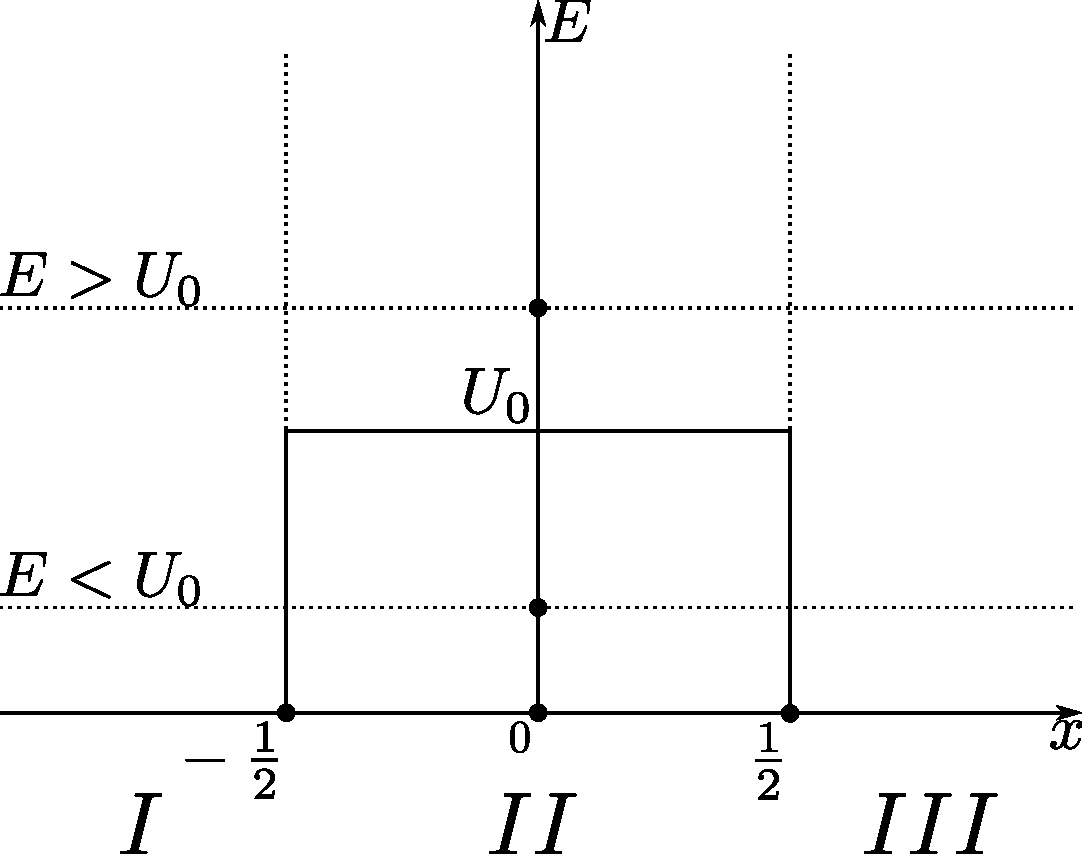
\includegraphics[width=1\linewidth]{48-02}
	\end{wrapfigure}
	Туннельный эффект: если барьер имеет конечную ширину, то коэффициент отражения меньше 1, а коэффициаент прохождения не равен нулю: вопреки классической механике, у электрона появляется отличная от нуля вероятность пройти через такой барьер.
	
	\textbf{Снова рассмотрим случай под кодовым именем А, где} $\xi < V_0$
	
	Область $\RNumb{1}$ :
	
	$$\psi_{\RNumb{1}} = A_1 e^{i k x} + B_1 e^{-i k x}$$
	
	$$k = \frac{\sqrt{2m\xi}}{\hbar}$$
	
	Область $\RNumb{2}$ :
	
	$$\psi_{\RNumb{2}} = A_2 e^{\kappa x} + B_1 e^{-\kappa x}$$
	 
	$$\kappa = \frac{\sqrt{2m(V_0 -\xi)}}{\hbar}$$
 
	Область $\RNumb{3}$ :
	
	$$\psi_{\RNumb{3}} = A_3 e^{i k x}$$
	
	Граничное условие:
	
	Для границы областей $\RNumb{1} \ и \ \RNumb{2}$
	
	\begin{equation*}
	\begin{cases}
		\psi_{\RNumb{1}} (-\frac{l}{2}) = \psi_{\RNumb{2}} (-\frac{l}{2}) \\\\
		\psi'_{\RNumb{1}} (-\frac{l}{2}) = \psi'_{\RNumb{2}} (-\frac{l}{2})
	\end{cases}	
	\end{equation*}

	Для границы областей $\RNumb{2} \ и \ \RNumb{3}$
	
	\begin{equation*}
		\begin{cases}
			\psi_{\RNumb{2}} (\frac{l}{2}) = \psi_{\RNumb{3}} (\frac{l}{2}) \\\\
			\psi'_{\RNumb{2}} (\frac{l}{2}) = \psi'_{\RNumb{3}} (\frac{l}{2})
		\end{cases}	
	\end{equation*}

	После вычислений получаем коэффициент проходимости электрона черех потенциальный барьер:
	
	$$D = \frac{4k^2 \kappa^2}{(k^2 + \kappa^2)^2 \sinh^2(\kappa l) + 4k^2\kappa^2}$$
	\\\\
	\textbf{Переходим к последнему случаю под кодовым именем Б, где} $\xi > V_0$
	\\\\
	Область $\RNumb{1}$ :
	
	$$\psi_{\RNumb{1}} = A_1 e^{i k_1 x} + B_1 e^{-i k_1 x}$$
	
	$$k_1 = \frac{\sqrt{2m\xi}}{\hbar}$$
	
	Область $\RNumb{2}$ :
	
	$$\psi_{\RNumb{2}} = A_2 e^{i k_2 x} + B_1 e^{-i k_2 x}$$
	
	$$k_2 = \frac{\sqrt{2m(\xi- V_0)}}{\hbar}$$
	
	Область $\RNumb{3}$ :
	
	$$\psi_{\RNumb{3}} = A_3 e^{i k_1 x}$$
	
	Граничные условия те же, что и в пункте А
	
	$$D = \frac{4k_1^2k_2^2}{(k_1^2-k_2^2)^2 \sin^2(k_2l)+4k_1^2k_2^2}$$
	\\\\
	$$\textbf{\textit{АЛЛИЛУЙЯ}}$$
\end{document}